\section{Parallel computing}
\subsection{Expressing parallelism}
\begin{tcolorbox}[violet] 
    There was different era of core computing, first the \important{simple core era}, we were executing one instruction per cycle.\\
    Then in \important{pre-multicore era}, we had one BIG fancy core:
    \begin{itemize}[left=10pt, label=\textbullet]
        \item A lot of budget on run a single instruction very fast, 
        \item More transistors, so faster branch predictor, larger cache hierarchy, etc\ldots
    \end{itemize}
    Finally, we are in the \important{multicore era}, more transistors, but in simple cores: each core is slower (around 25\%), but there is (for example) two cores \textrightarrow $\mathspace 2\cdot 0.75 = 1.5$.\\   
\end{tcolorbox}

    But now, we have to parallelize our code, either it will run on only one of the cores. There is different way expressing parallelism as programmer:
    \begin{itemize}[left=10pt, label=\textbullet]
        \item Use existing parallel code through libraries: Spiral, ScalAPACK,
        \item Writing in a parallel programming language: HPF, CAF, Java, Scala, 
        \item Writing in compiler directives: OpenMP, Intel TBB, 
        \item Writing using a threading library: MPI, PVM, Pthreads, 
        \item Domain Specific Languages (DSLs): Spiral, CUDA.
    \end{itemize}
    \newpage
    \textbf{PThreads:}
    \begin{codeCenter}
    \begin{Ccode}
void parallel_cbrt(float* v, float* result, int N) {
    pthread_t thread_id;
    my_args args;
    args.N = N/2;
    args.v = v;
    args.result = result;
   (*@ \colorbox{red!30}{pthread\_create(\&thread\_id, NULL, my\_thread\_start, \&args)} @*)
    my_cbrt(v + args.N, result + args.N, N - args.N);
   (*@ \colorbox{red!30}{pthread\_join(thread\_id, NULL);} @*)
}
    \end{Ccode}
    \end{codeCenter}
    
\textbf{OpenMP:} We can parallelize simply when loop iterations are independent of each other.
    \begin{codeCenter}
    \begin{Ccode}
void my_cbrt(float *v, float *result, int N) {
   (*@ \colorbox{red!30}{\#pragma omp parallel for} @*)
    for (int i = 0; i < N; ++i) {
    float x = 1.f;
    for (int j = 0; j < 10; ++j)
    x = (1.f / 3.f) * (2.f*x + v[i] / (x*x));
    result[i] = x;
    }
}    
    \end{Ccode}
    \end{codeCenter}
    
    \begin{tcolorbox}[vert]
        
    
        \hypertarget{simd}{}
        Another idea of \important{multicore era}, is the \important{SIMD processing}: Single Instruction, Multiple Data. We add ALUs to increase our compute capability, the idea is to transform a loop where there is an instruction repeated on a lot of different data into an single instruction on a vector of a lot of data, then for a simple for loop:
        \begin{codeCenter}
        \begin{Ccode}
for (int i = 0; i < 8; i++)
c[i] = a[i] + b[i];
        \end{Ccode}
        \end{codeCenter}
        We can compute this with one single operation of vector with the code:
        \begin{codeCenter}
        \begin{Ccode}
__m256 va = _mm256_load_ps(a);
__m256 vb = _mm256_load_ps(b);
__m256 vc = _mm256_add_ps(va, vb);
        \end{Ccode}
        \end{codeCenter}
        \lstinline!__m256! stand for the float type, the \lstinline!_mm256! is the size of the vector, here 256 bits (8 float) and the load/add is the operation of the function.\\
        GPUs are big SIMD processor!
    \end{tcolorbox}
\subsection{Principles of parallel computing}
    \begin{itemize}[left=10pt, label=\textbullet]
        \item Finding enough parallelism, 
        \item Division of work, 
        \item Scaling, 
        \item Communication and synchronization.
    \end{itemize}
    \begin{tcolorbox}[gris]
    \textbf{Finding enough parallelism:} this is all the Amdahl's law part.
    \end{tcolorbox}
    \begin{tcolorbox}[gris]
        \textbf{Division of work:}
        \begin{itemize}[left=10pt, label=\textbullet]
            \item Balance workload, give each parallel task the same rough amount of work.
            \item Reduce communication, computation is useful work, communication is overhead.
            \item Granularity, this is the ratio of computation to communication.
            \item Fine-grained parallelism: the idea is to split the work into very small tasks. There is not a lot of computation by thread but a lot of computation $\implies$ low granularity, but we need a fast communication favors: e.g. SIMD, GPU, \ldots 
            \item Coarse-grained parallelism: the idea is to split the work into big tasks. We have less cache and TLB misses and less communication, we can tolerate, but its harder to divide the work into equal time part.
        \end{itemize}
    \end{tcolorbox}

    \begin{tcolorbox}[gris]
        \textbf{Communication \& synchronization:}
        We will see three different model of communication/synchronization:
        \begin{itemize}[left=10pt, label=\textbullet]
            \item Message passing: the synchronization is at the I/O level, hadoop (e.g. Data center).
                \begin{itemize}[left=10pt]
                    \item There is completely different address spaces, threads communicate via sending/receiving message, the synchronization is implicit in messages. 
                    \item This is harder to program than shared memory, but more scalable.
                    \item Message passing is the most used communication system in data centers.
                \end{itemize}
                
            \item Shared memory: the synchronization is at the memory level, Scala (e.g. CPU). 
                \begin{itemize}[left=10pt]
                    \item Threads communicate by reading/writing to shared vars, that are like a big bulletin board (panneau d'affichage).
                    \item Any thread can read or write, communication is implicit in memory operations (no send/receive operations).
                    \item  Non-uniform memory access (NUMA): all processors can access any memory location, but cost of memory access is different for different processors.
                    \item Implementation and some example:
                            \begin{image}{Each thread has its own virtual address, but shared parts maps to the same physical location.}
                            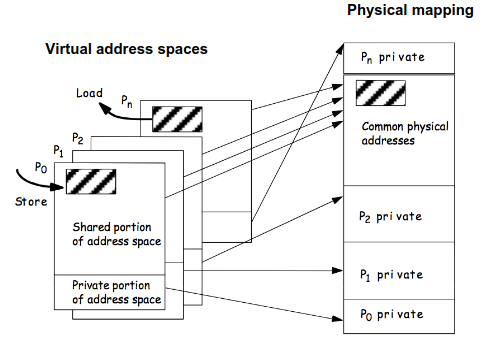
\includegraphics[width=6.5cm]{images/6.png}
                            \end{image}
                            \begin{image}{Any processor can directly reference any memory location (e.g. Intel Core i7 example (quad core)).}
                                \begin{center}
                            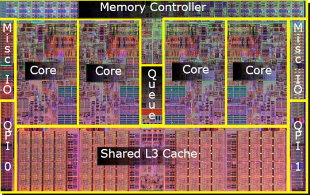
\includegraphics[width=4cm]{images/7.png}
                                \end{center}
                            \end{image}
                \end{itemize}
            \item Dataflow: the synchronization is at the processor level, TensorFlor (e.g. TPU).
                \begin{itemize}[left=10pt]
                    \item In data-parallel computation, communication and synchronization are implicit, since each processor works on a different part of the vector and synchronizes (or joins) at the end.                \end{itemize}
        \end{itemize}
    \end{tcolorbox}
